\documentclass[a4paper,11pt]{article} 

\usepackage[T1]{fontenc}
\usepackage[utf8]{inputenc}

\usepackage{multirow} 
\usepackage{booktabs} 
\usepackage{graphicx} 
\usepackage{setspace}
\usepackage[skip=6pt plus1pt, indent=0pt]{parskip}

\usepackage{float}
\usepackage{fancyhdr}

\usepackage{tcolorbox}
\usepackage{hyperref}
\hypersetup{
    colorlinks=true,
    linkcolor=blue,
    filecolor=magenta,      
    urlcolor=blue
}

\usepackage[margin=1in]{geometry}

\newcommand{\incode}[1]{
\begin{tcolorbox}[colback=blue!5!white, boxrule=0mm, sharp corners]
\texttt{#1}
\end{tcolorbox}
}

\newcommand{\note}[1]{\textit{\textcolor{gray}{#1}}}

\pagestyle{fancy} 
\fancyhf{} 
\lhead{Advanced Computer Networks 2022}
\rhead{Lin Wang, George Karlos, Florian Gerlinghoff} 
\cfoot{\thepage} 

\usepackage{minted}
\usepackage{wrapfig}

\begin{document}


\thispagestyle{empty} 

\begin{tabular}{@{}p{15.5cm}} 
{\bf Advanced Computer Networks 2022} \\
Vrije Universiteit Amsterdam \\ Lin Wang, George Karlos, Florian Gerlinghoff \\
\hline 
\\
\end{tabular} 

\vspace*{0.3cm} 

{\LARGE \bf Lab2: Data Center Network Topology (Report)} 

\vspace*{0.3cm} 

%============== Please do not change anything above ==============%

% Please modify this part with your group information
\begin{tcolorbox}[sharp corners, colback=blue!5!white]
\begin{tabular}{@{}ll}
\textbf{Group number:} & 9 \\
\textbf{Group members:} & Hsiang-ling Tai, Yung-sheng Tu, Sicheng Peng \\
\textbf{Slip days used:} & 0 \\
\textbf{Bonus claim:} & no
\end{tabular}
\end{tcolorbox}

\vspace{0.4cm}

% Please do not remove any of the section headings below

\section{Generating Fat-tree and Jellyfish Topologies}

\begin{enumerate}
    \item How to run our code
    \begin{itemize}
    First, install the required python packages by executing:
    \begin{minted}{bash}
    pip3 install -r lab2-group9/requirements.txt
    \end{minted}
    To generate and visualize fat-tree topology:
    \begin{minted}{bash}
    python3 lab2-group9/visualize_fattree.py
    \end{minted}
    To generate and visualize jellyfish topology:
    \begin{minted}{bash}
    python3 lab2-group9/visualize_jellyfish.py
    \end{minted}
    \textbf{NOTE}: The topology will pop up in the browser and also output to the current working directory as an HTML file.
    \end{itemize}
    \item How do we generate the topologies
    \begin{itemize}
        \item Fat-tree \\
        The number of ports is given, let \textit{k}=num\_ports, and there will be
        \begin{itemize}
            \item Create \textit{k} core switches instance
            \item Create \textit{k} pods and in every pod:
            \begin{itemize}
                \item Create \textit{$k/2$} upper-layer pod switches (aggregation switches) and \textit{$k/2$} lower-layer pod switches (edge switches)
                \item Link every upper-layer pod switch to every lower-layer pod switch
                \item Create \textit{$(k/2)^2$} hosts linked to lower-layer pod switches
            \end{itemize}
            \item Link core switches with upper-layer pod switches
        \end{itemize}
        \item Jellyfish \\
        A fully randomized topology with all switches randomly connected with each other. We take three steps to create:
        \begin{itemize}
            \item Node creation \\
            Create \textit{num\_switches} switches and \textit{num\_servers} hosts \\
            % Switches and host servers are created as nodes. 
            \item Switch interconnection \\
            Calculate the number of ports \textit{r} for each switch to connect with other switches according to the model: \textit{$num\_switch*(num\_ports-r)>=num\_servers$} \\
            Pairs of switch nodes are randomly selected and connected by adding an edge between them. A switch node is marked as stable when it has no more free ports to connect with other switches. Repeat this process until all switches are stable.
            If there is any switch $s_{invalid}$ has >= 2 free ports when all switches are stable, remove one random edge which links two random switches $s_1$ and $s_2$, and then link $s_{invalid}$ to $s_1$ and $s_2$ by adding two edges.
            \item Host-switch connection \\
            Uniformly distribute the hosts to switches until all hosts are connected to a switch.
        \end{itemize}
        The jellyfish topology is completed when all host servers and switches are connected, and no switch has >= 2 free ports.
        
    \end{itemize}
    
%    \newpage
    \vspace{3mm}
    \item Example topologies
\end{enumerate}
    \vspace{5mm}
    % \begin{figure}[!htb]
    % \centering
    % 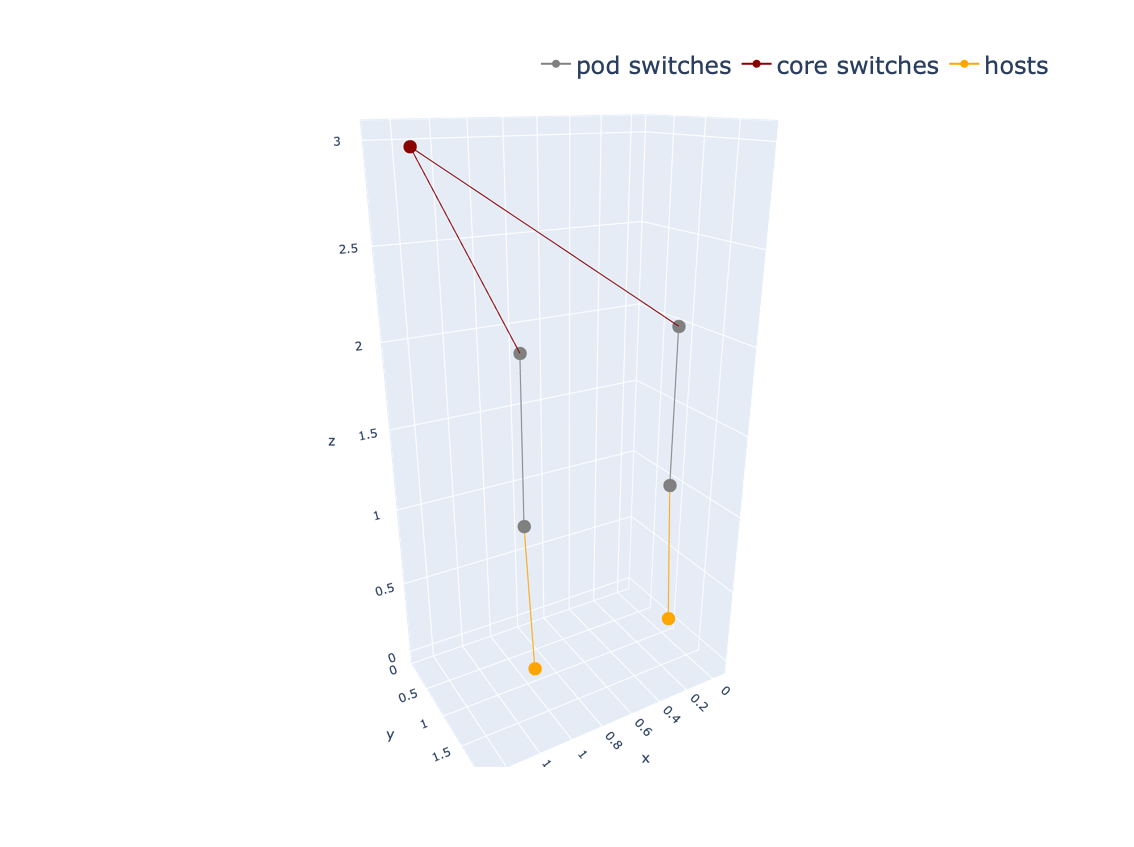
\includegraphics[width=0.8\textwidth]{fattree_k2.png}
    % \caption{Fat-tree Topology with k=2}
    % \label{fig:fatk2}
    % \end{figure}
    % \begin{figure}[!htp]
    % \centering
    % 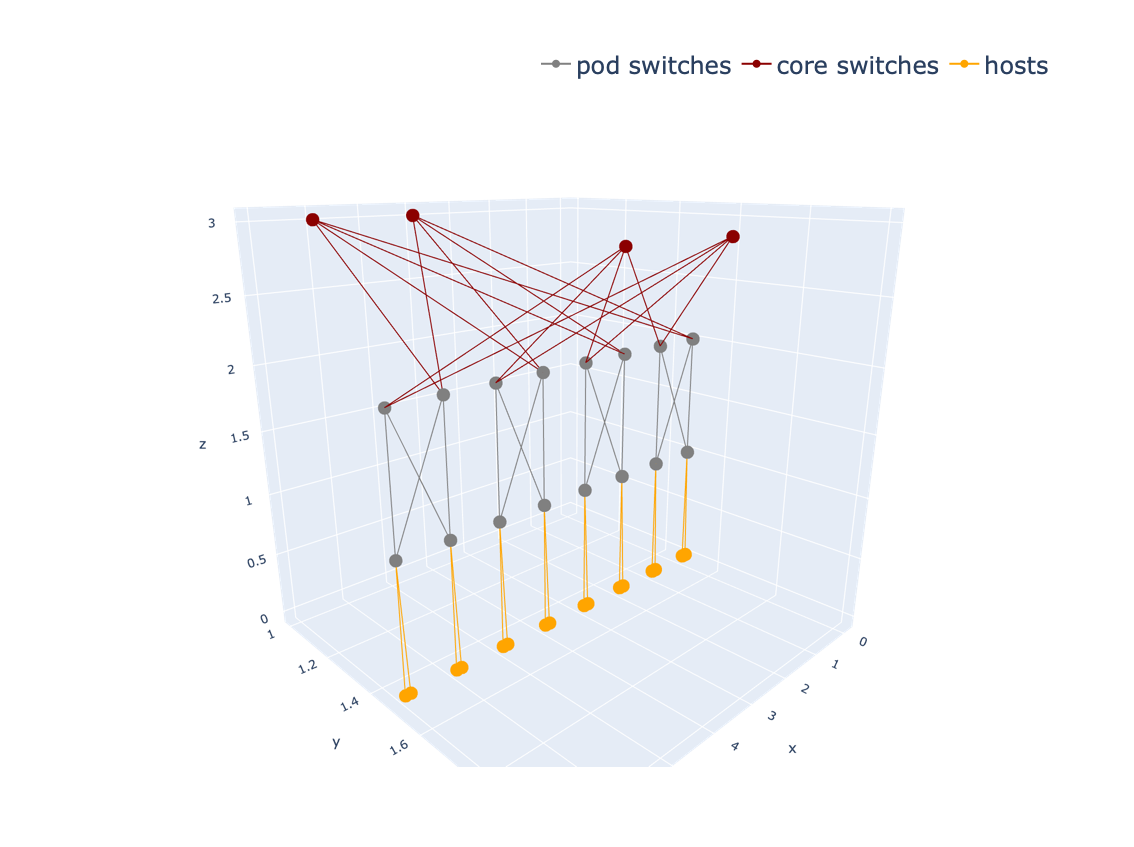
\includegraphics[width=0.9\textwidth]{fattree_k4.png}
    % \caption{Fat-tree Topology with k=4}
    % \label{fig:fatk4}
    % \end{figure}
    \begin{figure}[htbp]
    \centering
    \begin{minipage}[t]{0.48\textwidth}
    \centering
    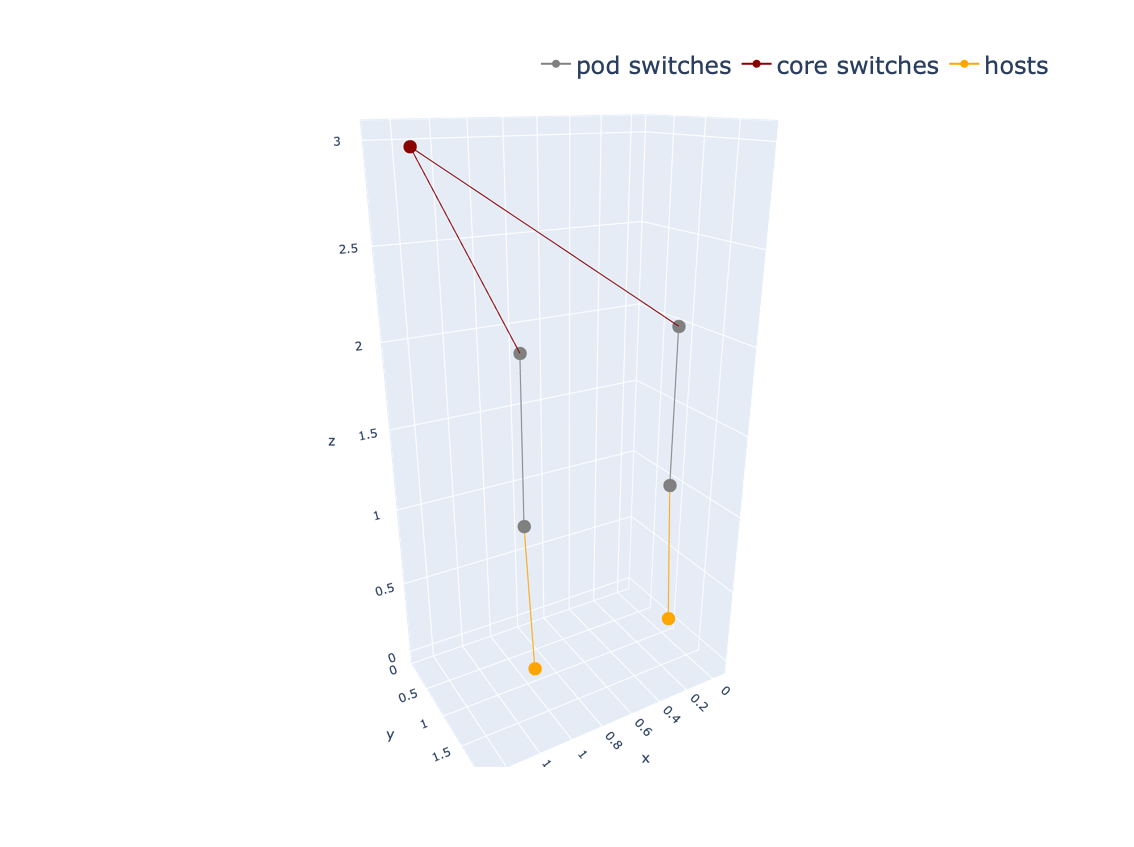
\includegraphics[width=8cm]{fattree_k2.png}
    \caption{Fat-tree with 2 servers, 5 switches, 2 ports}
    \end{minipage}
    \begin{minipage}[t]{0.48\textwidth}
    \centering
    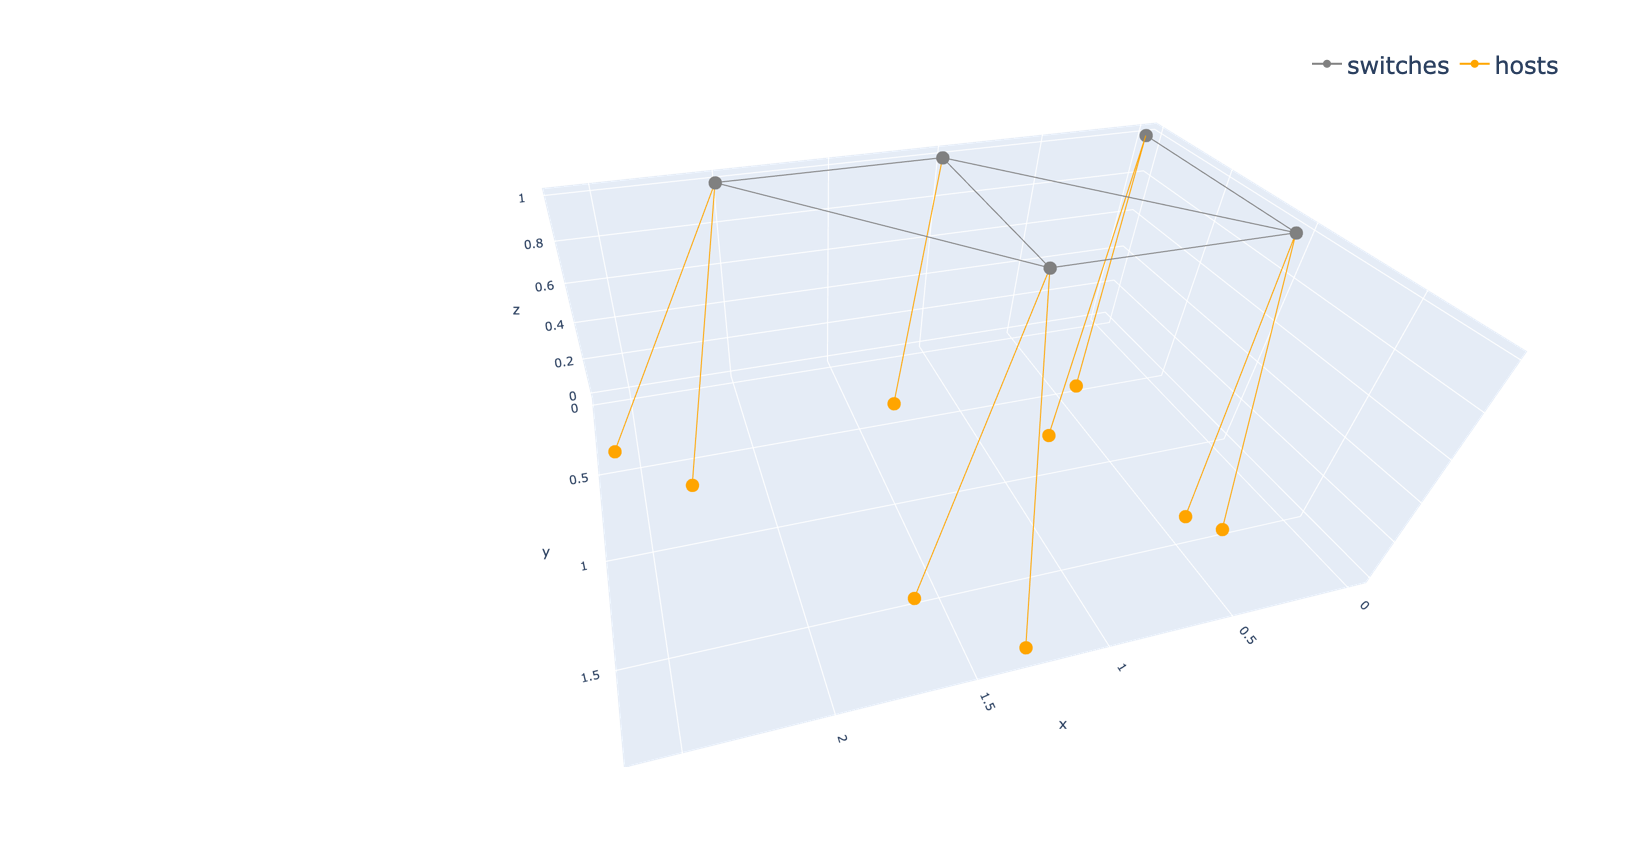
\includegraphics[width=8cm]{jellyfish_k2.png}
    \caption{Jellyfish with 10 servers, 5 switches, 5 ports}
    \end{minipage}
    \end{figure}
    \begin{figure}[htbp]
    \centering
    \begin{minipage}[t]{0.48\textwidth}
    \centering
    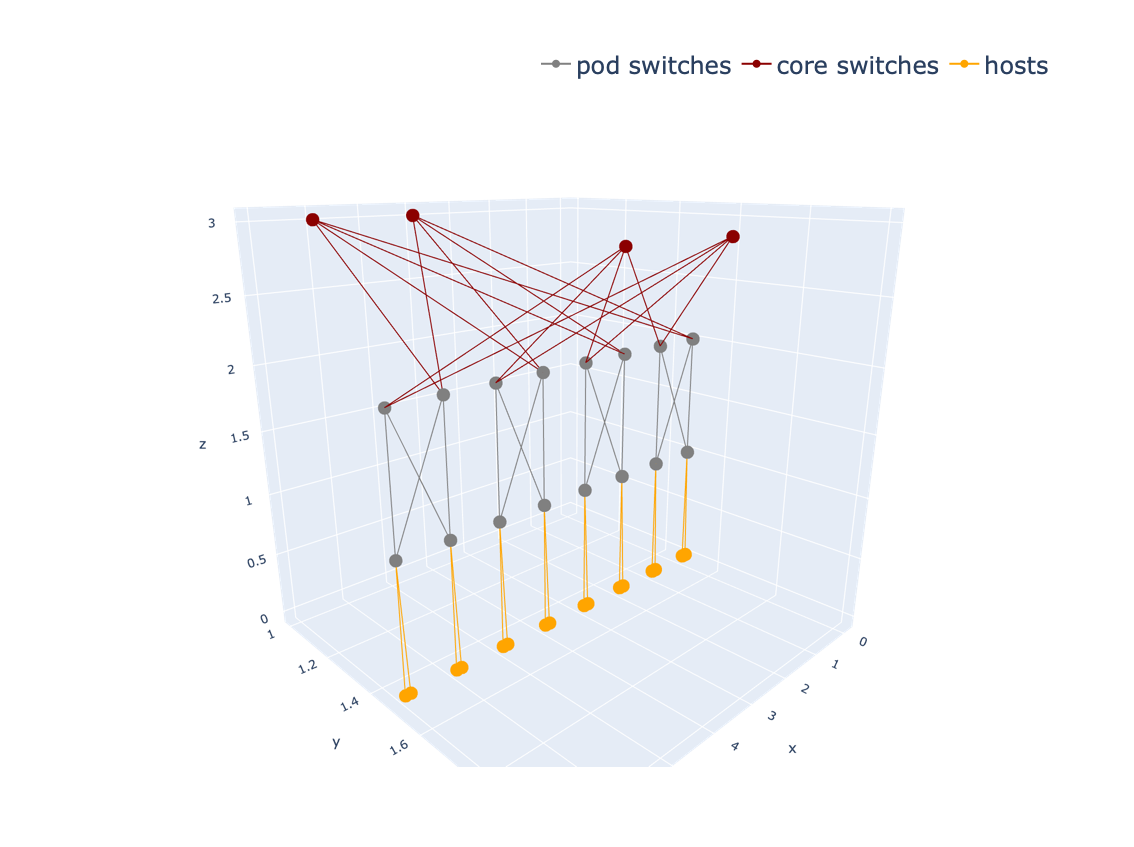
\includegraphics[width=8cm]{fattree_k4.png}
    \caption{Fat-tree with 16 servers, 20 switches, 4 ports}
    \end{minipage}
    \begin{minipage}[t]{0.48\textwidth}
    \centering
    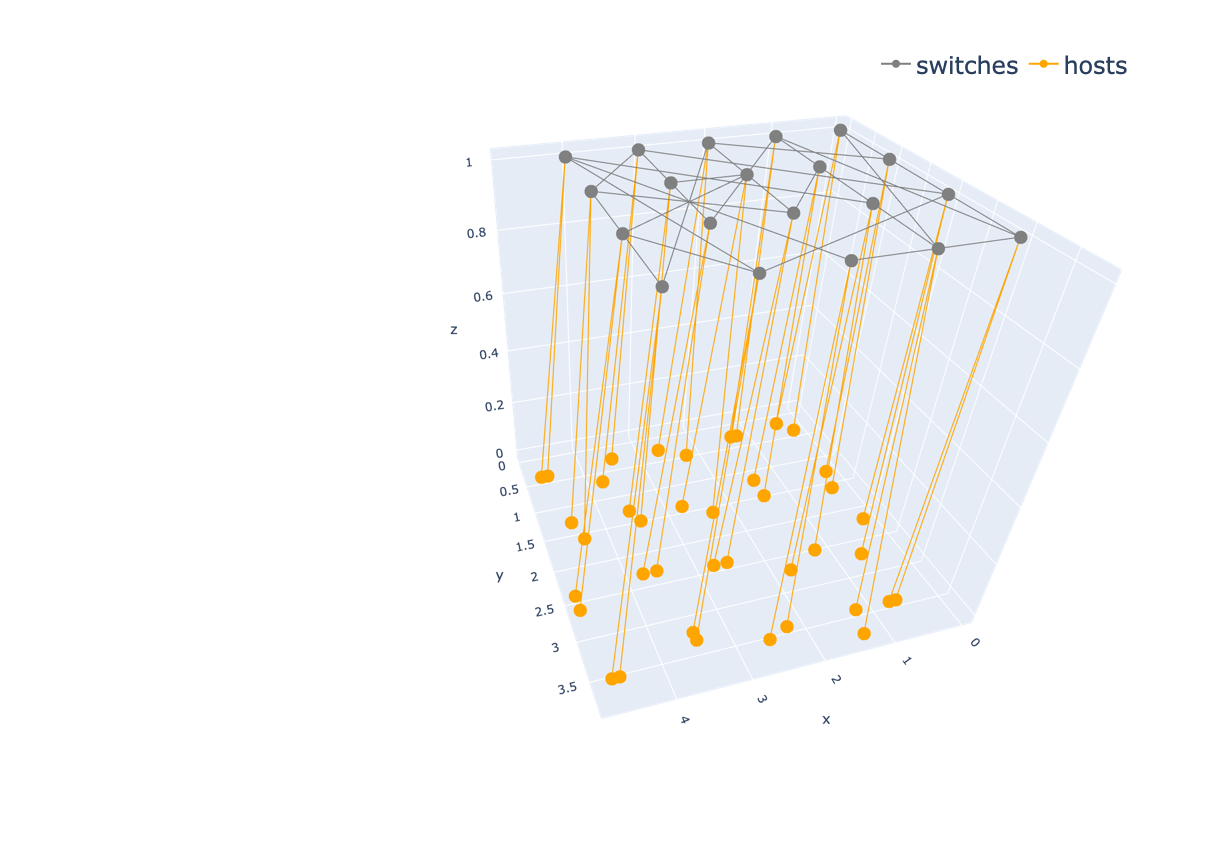
\includegraphics[width=8cm]{jellyfish_k4.png}
    \caption{Jellyfish with 40 servers, 20 switches, 5 ports}
    \end{minipage}
    \end{figure}
    \begin{figure}[htbp]
    \centering
    \begin{minipage}[t]{0.48\textwidth}
    \centering
    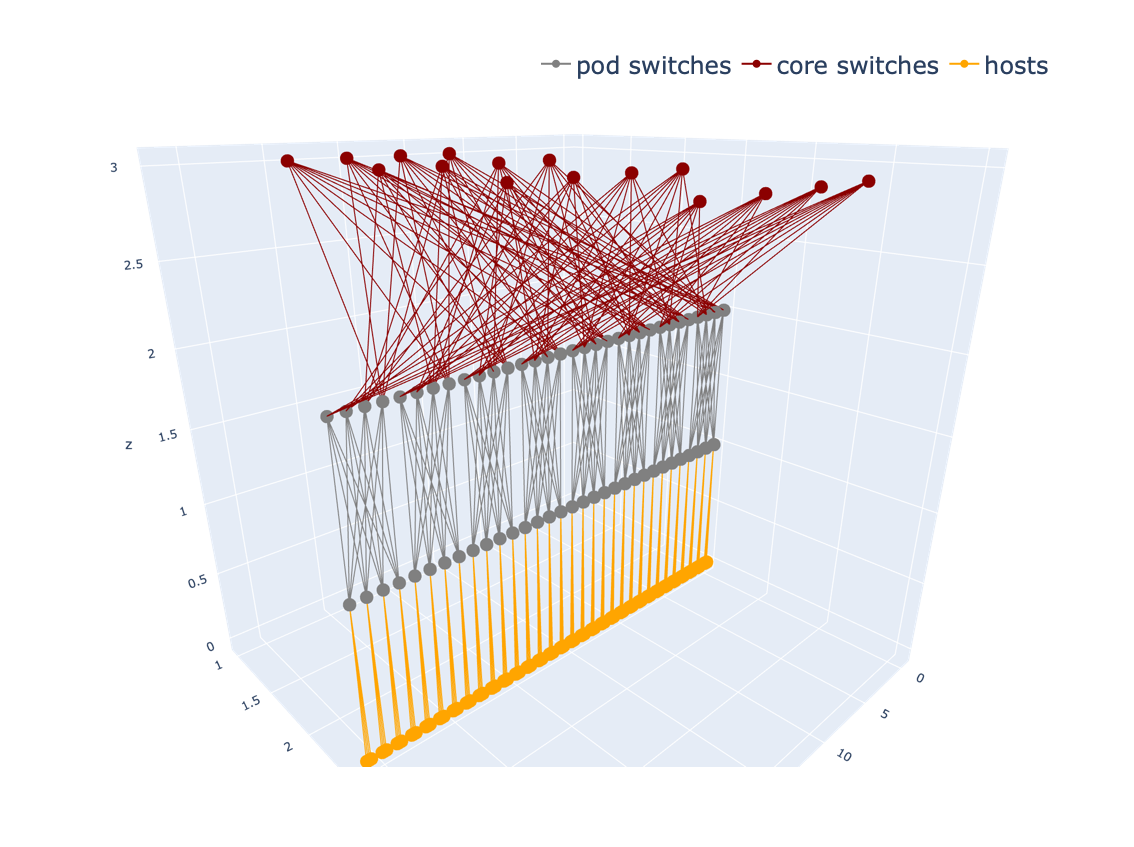
\includegraphics[width=8.3cm]{fattree_k8.png}
    \caption{Fat-tree with 128 servers, 80 switches, 8 ports}
    \end{minipage}
    \begin{minipage}[t]{0.48\textwidth}
    \centering
    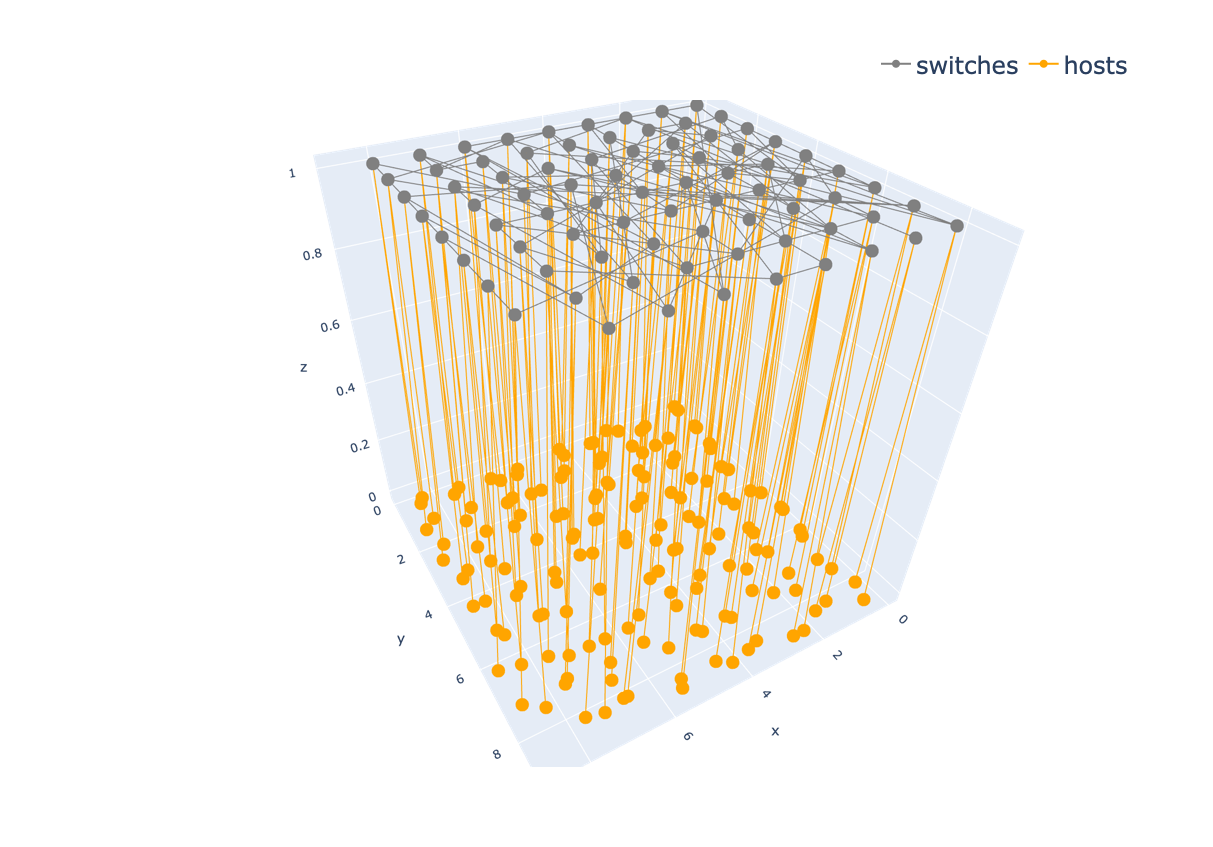
\includegraphics[width=8.3cm]{jellyfish_k8.png}
    \caption{Jellyfish with 160 servers, 80 switches, 5 ports}
    \end{minipage}
    \end{figure}
    
    % \vspace{5mm}
    
    % \begin{figure}[!htp]
    % \centering
    % 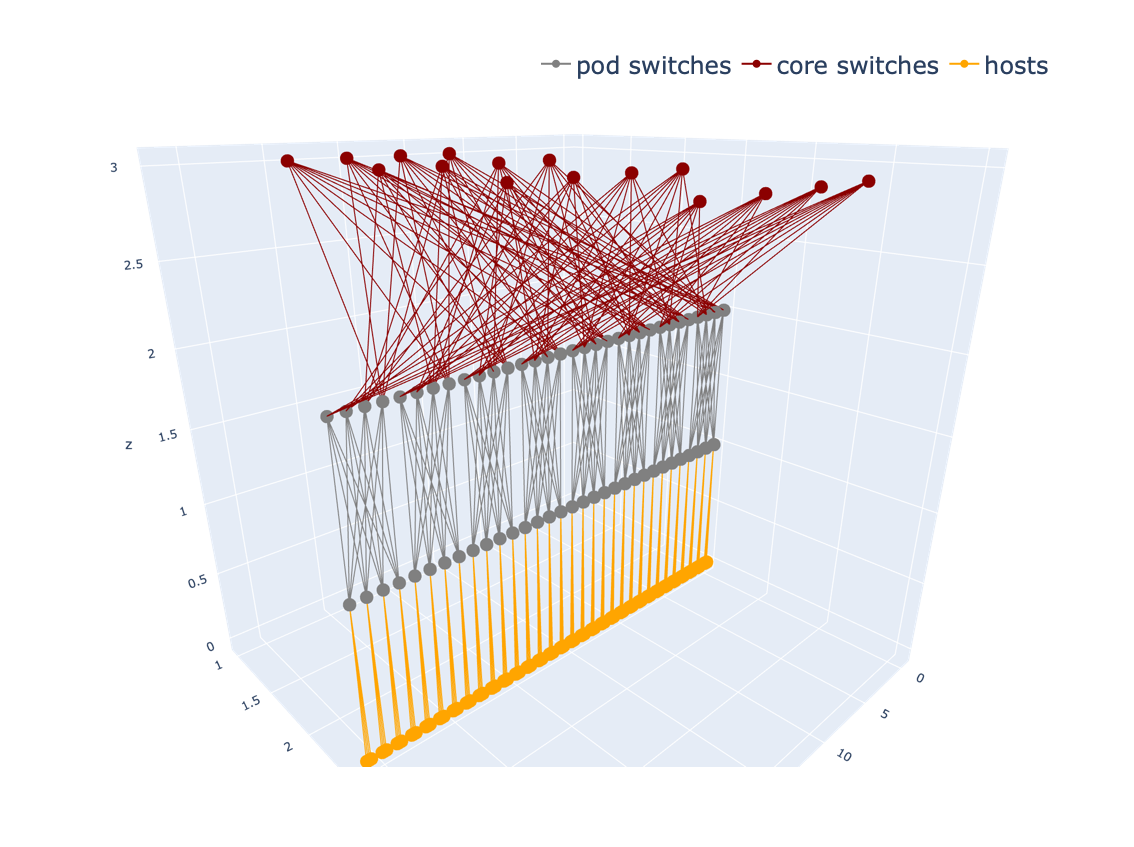
\includegraphics[width=0.6\textwidth]{fattree_k8.png}
    % \caption{Fat-tree Topology with k=8}
    % \label{fig:fatk8}
    % \end{figure}
    % \begin{wrapfigure}{i}{\textwidth}
    % 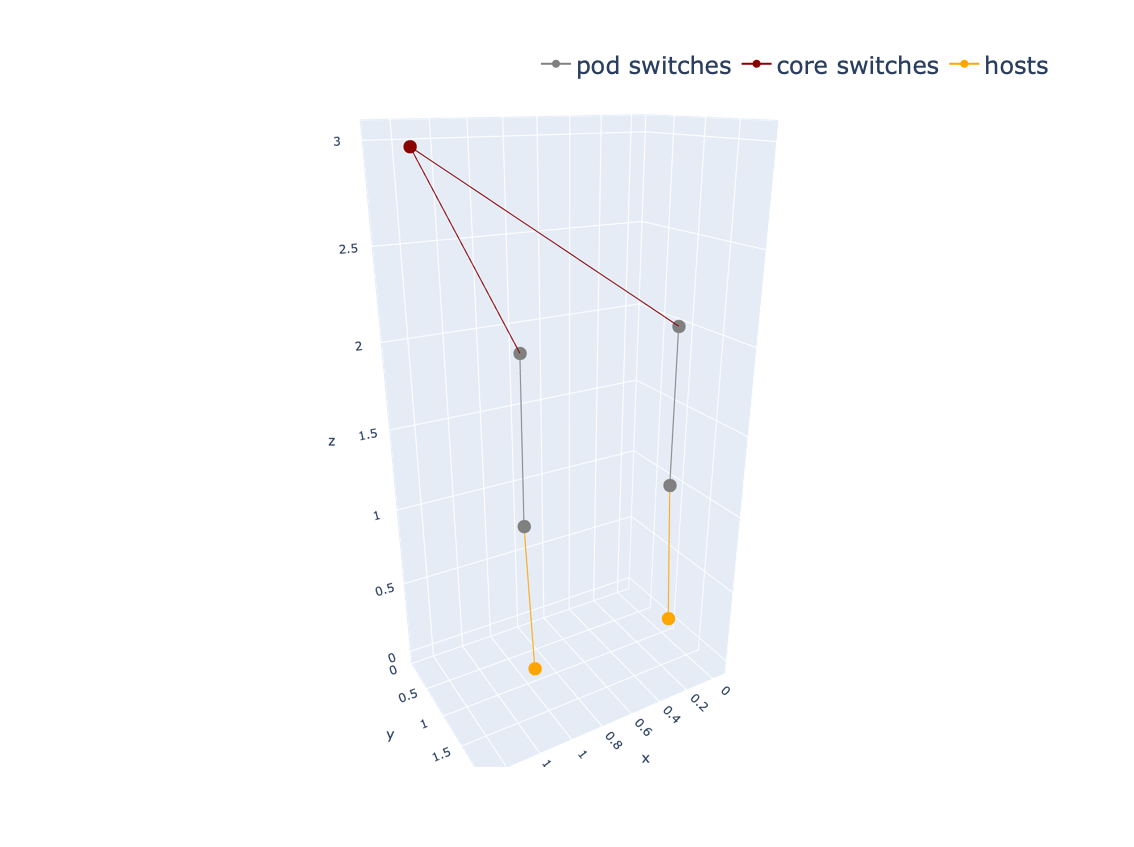
\includegraphics[width=0.9\textwidth]{fattree_k2.png} 
    % \caption{Caption1}
    % \label{fig:wrapfig}
    % \end{wrapfigure}
    % \begin{wrapfigure}{i}{\textwidth}
    % 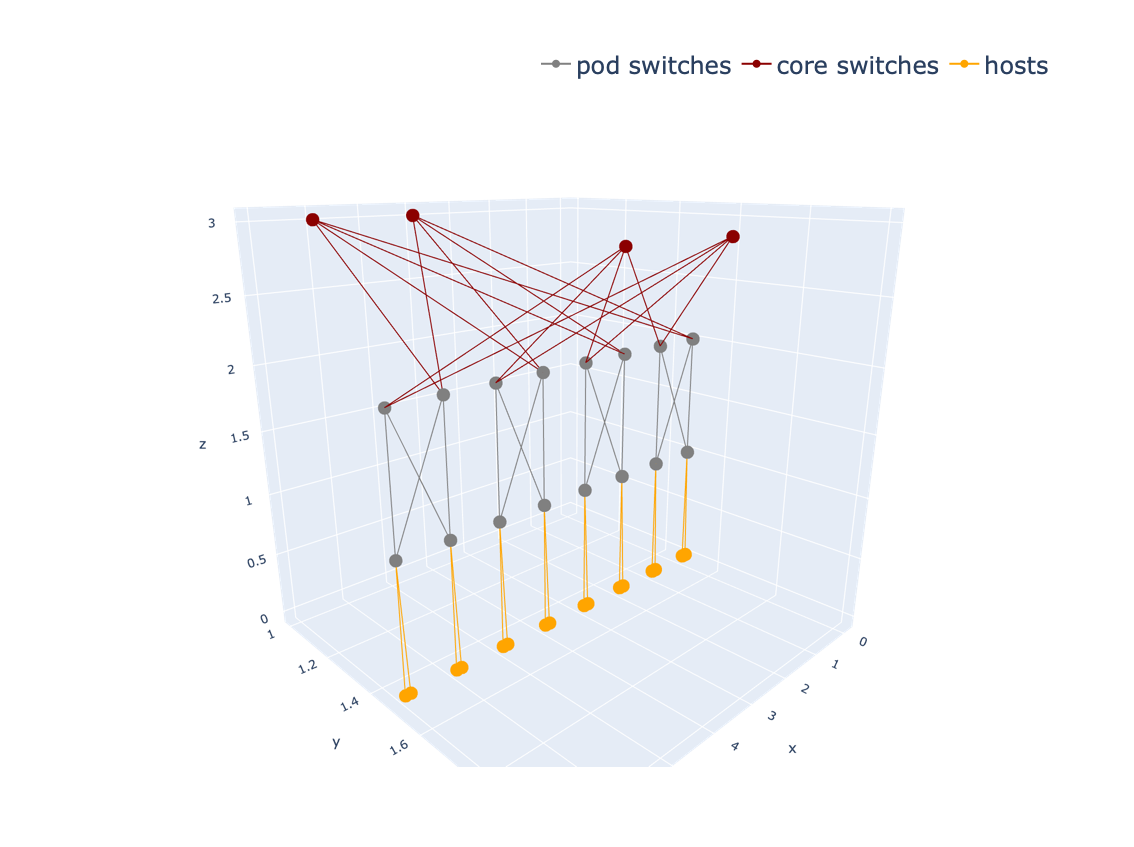
\includegraphics[width=0.9\textwidth]{fattree_k4.png} 
    % \caption{Caption1}
    % \label{fig:wrapfig}
    % \end{wrapfigure}


\newpage

\section{Comparing the Properties of Fat-tree and Jellyfish}
\begin{enumerate}
    \item How to run our code
    \begin{itemize}
    First, install the required python packages by executing:
    \begin{minted}{bash}
    pip3 install -r lab2-group9/requirements.txt
    \end{minted}
    To reproduce figure 1(c):
    \begin{minted}{bash}
    python3 lab2-group9/reproduce_1c.py
    \end{minted}
    To reproduce figure 9: ( NOT DONE YET )
    \begin{minted}{bash}
    python3 lab2-group9/reproduce_9.py
    \end{minted}
    \textbf{NOTE}: The figure will pop up in the browser and also output to the current working directory as an HTML file.
    \end{itemize}
    \item How do we reproduce the figure
    \begin{itemize}
        \item Reproduce figure 1(c)
            \begin{itemize}
            \item Generate fat-tree and jellyfish topologies
            \item Get all host-to-host shortest path lengths by Dijkstra's Algorithm
            \item Calculate the number of every kind of path length, and divide with the number of all path
            %\item Calculate the shortest paths with Dijkstra's Algorithm
            %\item Simultaneously, store the all the shortest paths between the servers
            %\item Categorise them according to their length
            \end{itemize}
            \textbf{NOTE}: Jellyfish run 3 trials to get average
        \item Reproduce figure 9\\
            NOT DONE YET
    \end{itemize}

    % \vspace{2mm}
    \newpage
    \item Figures
    \begin{figure}[!htp]
    \centering
    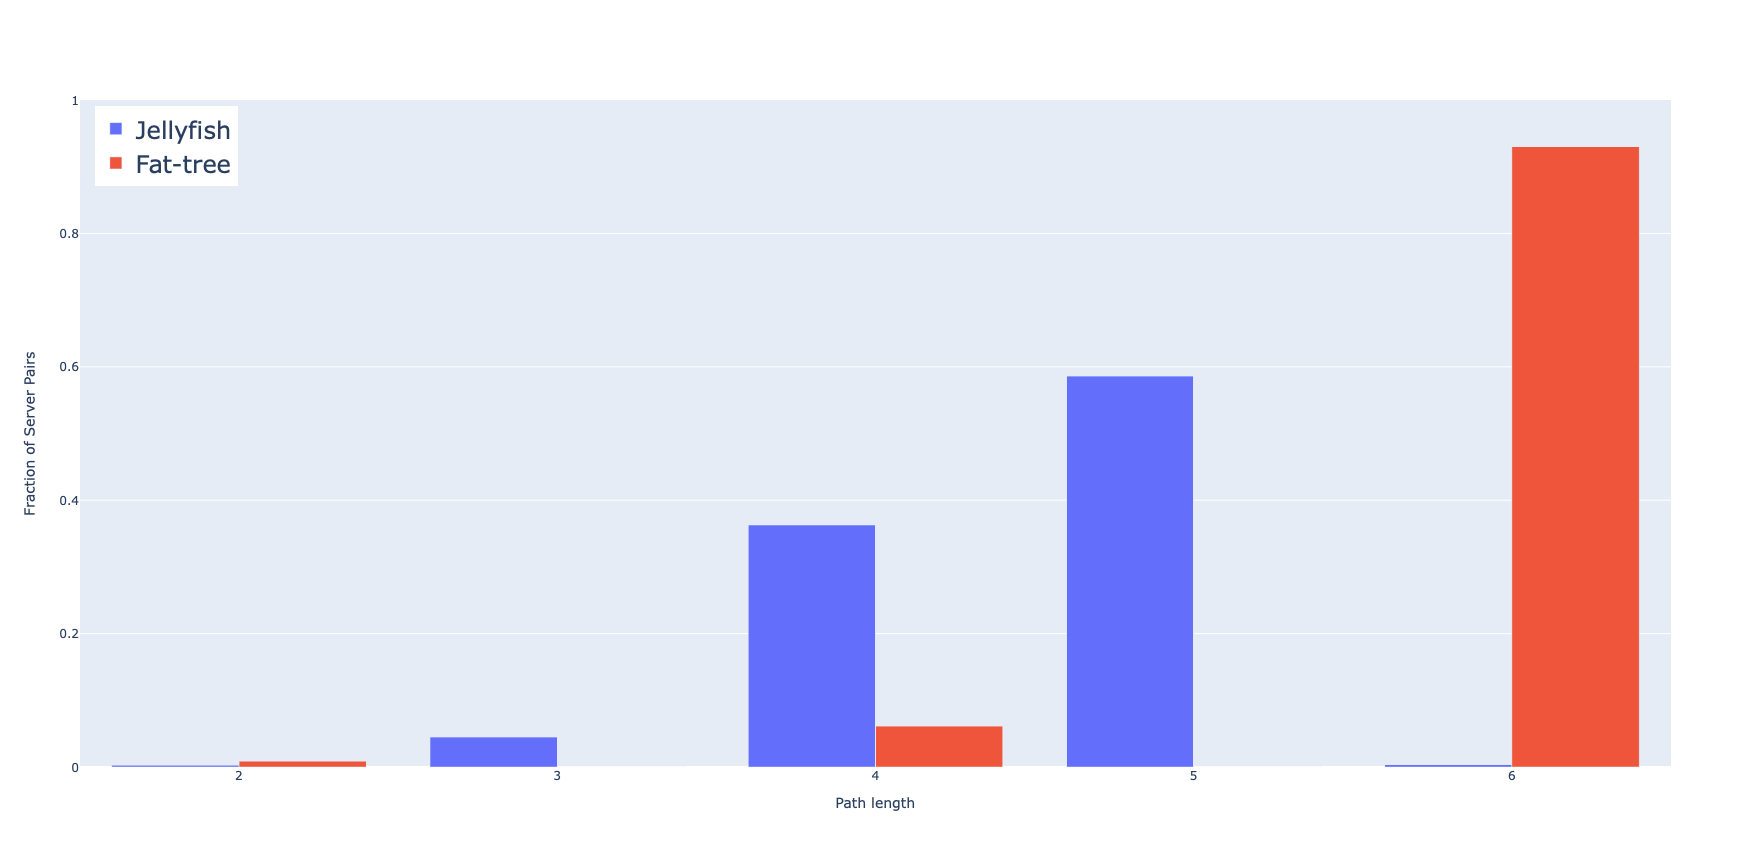
\includegraphics[width=0.9\textwidth]{reproduce_1c.png}
    \caption{Reproduced Figure (1c)}
    \label{fig:rf1c}
    \end{figure}
    \item Explanation for the comparison \\

    Figure \ref{fig:rf1c} has the same pattern as Figure 1c. Figure 1c shows that a few host servers of jellyfish topology can reach each other in two hops, while there is none in Figure  \ref{fig:rf1c}. A possible reason would be that in the reproduce experiment, we have set a limit that every switch can only connect to a maximum of one host server, while the experiment of Figure 1c may not have this limit.
\end{enumerate}

% Start your writing here, feel free to include subsections to structure your report if needed
% Please remove the note below in your submission
% \note{Please include at least the following: (1) how we should run your code, (2) your general approach to reproducing the figure, (3) the figure you have reproduced, and (4) explanation for the comparison (e.g., reason about any differences to the original figures in the paper, if any).}

\end{document}
